% =============================================================================
%  Ask the Sensors -- Technical Report
%  CS60055 Ubiquitous Computing, Hackathon Challenge 1
%
%  Compiles with pdflatex (standard packages only; no shell-escape needed):
%      pdflatex report && pdflatex report
%  Figures are expected in ./figures/ (copied from outputs/figures/).
% =============================================================================
\documentclass[11pt,a4paper]{article}

\usepackage[T1]{fontenc}
\usepackage[utf8]{inputenc}
\usepackage{lmodern}
\usepackage[margin=1in]{geometry}
\usepackage{graphicx}
\usepackage{booktabs}
\usepackage{amsmath}
\usepackage{microtype}
\usepackage{caption}
\usepackage{enumitem}
\usepackage{xcolor}
\usepackage{tabularx}
\usepackage{array}
\usepackage[colorlinks=true,linkcolor=black,citecolor=black,urlcolor=blue]{hyperref}

\captionsetup{font=small,labelfont=bf}
\setlist{nosep,leftmargin=1.4em}
\newcommand{\code}[1]{\texttt{\small #1}}
\newcolumntype{R}{>{\raggedleft\arraybackslash}X}

\title{\textbf{Ask the Sensors}\\[2pt]
\large Grounded, Explainable Activity Question Answering\\
\large from Wearable Accelerometer and Gyroscope Signals}

\author{%
  \textit{Team} \textbf{$\langle$TEAM NAME$\rangle$} \\[4pt]
  $\langle$Member 1 Name$\rangle$ ($\langle$Roll$\rangle$) \quad
  $\langle$Member 2 Name$\rangle$ ($\langle$Roll$\rangle$) \quad
  $\langle$Member 3 Name$\rangle$ ($\langle$Roll$\rangle$) \\[4pt]
  CS60055 Ubiquitous Computing --- Hackathon Challenge 1 \\
  Indian Institute of Technology Kharagpur%
}
\date{\today}

\begin{document}
\maketitle

\begin{abstract}
\noindent
We present \emph{Ask the Sensors}, a system that answers natural-language questions
about human activity directly from raw wearable inertial signals, and that cites the
specific stretch of signal supporting every answer. The design follows one invariant:
\textbf{evidence flows upward and language only selects it}. Signal processing and a
classifier produce a timeline of activity bouts; a question is reduced to a structured
\emph{intent} and answered by arithmetic over that timeline; a small language model is
consulted only to interpret unfamiliar \emph{wording}, never to produce a fact. Over
five user-disjoint folds of the ExtraSensory corpus (35 users, 165{,}787 windows,
7~activity classes) the recogniser reaches $0.703 \pm 0.032$ window accuracy, and
1{,}159 generated question--answer cases score $0.567$ answer accuracy and $0.348$
\emph{grounded} accuracy --- the stricter number, which additionally requires the cited
interval, modality and channels to be correct. An accuracy-versus-overhead study
identifies an edge operating point that is $9.6\times$ smaller on disk for 14 accuracy
points, and isolates the language model's cost as roughly $24{,}000\times$ that of
classifying a window, which is precisely why it sits behind a deterministic fast path.
\end{abstract}

\vspace{-0.5em}
\section{The problem, as we framed it}

The brief asks for a system that takes a wearable sensor recording and a question in
plain English, and returns not just an answer but the evidence for it: timestamps,
sensor modality, channels, and an explanation. Four tasks are specified, in increasing
difficulty: (1)~activity identification and binary verification, (2)~temporal and
quantitative reasoning (durations, counts, comparisons), (3)~evidence grounding
(\emph{when} did it happen), and (4)~open-world reasoning about behaviour phrased in
words the system was never given as a class label.

Three framing decisions shaped everything that followed.

\paragraph{The deliverable is evidence, not a label.} A classifier that is right about
the activity but cites the wrong 15~seconds has not answered the question as asked. We
therefore made the \emph{interval} --- not the per-window prediction --- the system's
unit of output, and we score ourselves primarily on \textbf{grounded accuracy}: the
answer must be correct \emph{and} the cited interval must overlap the truth at
$\mathrm{IoU} \ge 0.5$ \emph{and} the modality and channels must match. This number is
always lower than answer accuracy, and it is the one we ask to be judged on.

\paragraph{A language model must not be allowed to invent a measurement.} The obvious
architecture --- feed a window summary to an LLM and let it answer --- fails the brief
at its core, because a fluent model will produce a plausible timestamp whether or not
one exists. We inverted the relationship: the language model receives a \emph{menu of
real intervals} produced by the signal layers and may only refer to them by index. A
citation not on the menu is discarded rather than rendered. An answer from our system
can be wrong; it cannot be \emph{unfounded}.

\paragraph{Generalisation means a new person, not a new window.} Windows from one
subject are strongly autocorrelated, so a random train/test split leaks a subject
across both sides and inflates accuracy substantially. Every number in this report comes
from \textbf{user-disjoint} folds: no user appears in both the training and the
evaluation side of any fold. This costs us perhaps 20--30 accuracy points against a
window-shuffled split, and is the only honest way to report the quantity the brief
cares about --- how the system behaves on someone it has never seen.

\paragraph{Data.} ExtraSensory \cite{vaizman2017} --- in-the-wild smartphone and
smartwatch recordings from 60 users over days, with per-minute labels. We use the raw
accelerometer and gyroscope captures (not the authors' precomputed features) for 35
users, and the seven classes the brief names: \code{lying\_down}, \code{sitting},
\code{standing\_in\_place}, \code{standing\_and\_moving}, \code{walking},
\code{running}, \code{bicycling}. Two properties of this corpus drive the design: the
sensors are sampled on \textbf{separate, drifting clocks}, and the recording is
\textbf{intermittent} --- roughly 15~seconds of signal are captured in every 60~seconds
of wall-clock time.

\section{Design and the reasons for it}

The system is four layers with a decoder inserted between the second and third. Each
layer consumes only the layer below and adds exactly one kind of structure; nothing
skips a layer, and nothing asserts a fact the layer below did not measure.

\begin{center}
\small
\begin{tabular}{@{}ll@{}}
\toprule
\textbf{Layer} & \textbf{Adds} \\
\midrule
L1 \ \code{preprocess.py} & clock-true resampling to a 25\,Hz grid $\rightarrow$ 15\,s windows of 6 channels \\
L2a \ \code{features.py}  & 40 physically interpretable features per window \\
L2b \ \code{context.py}   & $+63$ temporal-context features $=103$ \\
L2 \ \code{recognise.py}  & hierarchical XGBoost $\rightarrow$ calibrated $P(\text{activity} \mid \text{window})$ \\
L2c \ \code{decode.py}    & time-aware HMM $\rightarrow$ one coherent label per window \\
L3 \ \code{timeline.py}   & windows $\rightarrow$ bouts $\rightarrow$ \code{Timeline} (\emph{the evidence store}) \\
L4 \ \code{intent.py}, \code{answer.py} & question $\rightarrow$ \code{Intent} $\rightarrow$ \code{Answer} $+$ citations \\
L4b \ \code{slm.py} & unfamiliar wording only: Qwen2.5-3B as a \emph{parser} \\
\bottomrule
\end{tabular}
\end{center}

\subsection{L1: resample by the sensor's clock, not by sample index}

ExtraSensory's accelerometer and gyroscope run on independent clocks that drift. The
measured inter-sample interval ranges from $0.024$\,s to $0.077$\,s across devices, so a
fixed block of 800 samples spans anywhere from $\sim$9\,s to $\sim$25\,s depending on
whose phone it came from. Two consequences follow, and both are silent:

\begin{enumerate}
\item \textbf{Index-based windowing distorts time.} The same ``window'' means a
different number of seconds per user, which corrupts every frequency-domain feature ---
a 2.0\,Hz cadence is read as 2.3\,Hz. A regression test
(\code{tests/test\_preprocess.py}) pins exactly this error.
\item \textbf{Zipping the two sensors by index misaligns them} by a growing offset,
quietly destroying every cross-modal feature.
\end{enumerate}

So both streams are interpolated onto one \emph{absolute} time grid at exactly
$0.04$\,s per sample, over only the interval both sensors actually observed. A window is
375 samples $=15$\,s. Any window containing a sensor gap wider than
$\mathrm{MAX\_SAMPLE\_GAP\_S}=0.5$\,s is \textbf{rejected, not interpolated across},
with a recorded reason. Rejection over interpolation is a direct consequence of the
grounding requirement: interpolated signal would be manufactured, and would then be
cited as evidence. This layer is why our timestamps are trustworthy enough to print.

\subsection{L2a: features chosen to be nameable}

Forty features per window, selected so that a human can read the \emph{explanation}
rather than only the verdict. A Butterworth low-pass at $0.3$\,Hz separates
acceleration into a gravity component --- giving \textbf{device tilt}, which is what
distinguishes lying from upright --- and a body-acceleration component, giving
\textbf{motion energy}. Autocorrelation recovers \textbf{cadence}: $1.5$--$2.2$\,Hz is
walking, $2.5$--$3.5$\,Hz is running. The rest are spectral entropy, four band powers,
jerk, crest factor, zero-crossing rate, gyroscope rotation magnitude and axis
dominance, and accelerometer--gyroscope correlation.

This choice has a cost in raw accuracy relative to a learned representation, and it buys
the thing the brief actually asks for: an answer can say \emph{``a 2.5\,Hz cadence and a
gravity vector 85$^\circ$ from the device axis''} instead of \emph{``the classifier said
so.''} Every phrase in an explanation traces to one of these 40 numbers.

\subsection{L2b: temporal context --- the single largest accuracy lever}

A single 15-second window of stillness genuinely \emph{cannot} distinguish lying from
sitting; the information is not present. A stretch of such windows can. We add
time-bounded rolling mean and standard deviation at four radii ($\pm 2, 5, 15, 30$
windows $\approx \pm 2, 5, 15, 30$ minutes), previous/next values and deltas, over the
five base channels that each answer a different physical question (motion energy,
posture, rhythm, rotation, spectral order), plus gap sizes and a neighbour count:
63 features.

Two guards matter. Neighbours more than \textbf{40 minutes} away are ignored even when
adjacent in the array --- recordings are intermittent, so the previous row may be from
yesterday, and averaging it in would invent continuity that never existed. And context
never crosses a recording boundary. \code{tests/test\_context.py} asserts both.

This is worth \textbf{$+0.20$ window accuracy} ($0.457 \rightarrow 0.660$), by far the
largest single gain in the system. For the honest single-window case (Task~1 on one
isolated \code{.dat} file) \code{augment\_isolated()} supplies neutral context and
scores $0.506$; the gap between those numbers \emph{is} the value of context, stated
rather than hidden.

\subsection{L2: a hierarchy of three classifiers, not one seven-way model}

\begin{center}
\small
\begin{tabular}{@{}ll@{}}
\code{stage1} & binary: \textbf{static vs.\ dynamic} \\
\quad $\vdash$ \code{stage2a} & \code{lying\_down} / \code{sitting} / \code{standing\_in\_place} \\
\quad $\vdash$ \code{stage2b} & \code{standing\_and\_moving} / \code{walking} / \code{running} / \code{bicycling} \\
\end{tabular}
\end{center}

The static/dynamic boundary is the most reliable discrimination in accelerometry, so it
is decided first, on its own, and never revisited; the harder within-branch decisions
are then made by specialists that are not also trying to learn the easy split.
Probabilities compose as $P(\text{leaf}) = P(\text{branch}) \times P(\text{leaf} \mid
\text{branch})$, are renormalised, and are then passed through a \emph{fitted
temperature} ($\approx 0.86$--$1.27$ by fold). Calibration is not cosmetic here: the
HMM below consumes these as likelihoods, not as \code{argmax} decisions, so
overconfident probabilities would defeat the decoder.

Gradient-boosted trees (XGBoost) on interpretable features were chosen \emph{by
measurement}. Our first exploratory models, trained on a 6-user subset with a single
held-out test user, were a 300-tree random forest ($0.532$ accuracy, $0.257$ macro-F1)
and a 320k-parameter 1-D CNN over raw windows ($0.328$ accuracy, $0.218$ macro-F1). The
CNN lost, and lost in an instructive way: with 82 running and 106 bicycling windows in
the training set, it collapsed onto the majority postures, and it could not have
explained itself if it had won. Physics-based features plus boosting dominate at this
data scale, and they keep the explanation.

\paragraph{The derived seventh class.} The brief asks for \code{standing\_in\_place} and
\code{standing\_and\_moving}; ExtraSensory annotates a single \code{OR\_standing}.
Rather than ask a tree to learn a boundary its labels do not contain, \code{StandingSplit}
divides that class on measured body-acceleration energy at a threshold fitted
\emph{on training users only} ($\approx 0.0136$--$0.0157$\,g by fold). Rows carry a
provenance marker (\code{annotated} vs.\ \code{derived}) so this class can always be
scored separately from the five the corpus actually annotates.

\subsection{L2c: a time-aware HMM, because flicker becomes false evidence}

Per-window predictions flicker. In a grounded system this is worse than a plain accuracy
loss: a single misread window inside a ten-minute walk creates a spurious one-window
``bout'' that the interface layer would then \emph{cite as evidence}. The decoder imposes
temporal coherence.

Transitions are \textbf{time-aware}. Because rejected windows leave gaps, the step
between consecutive rows is not constant, so a per-minute transition matrix $T$ is
raised to the power $\Delta t / 60$ via a generator matrix rather than applied as a
fixed step. The practical effect is that a multi-hour dropout \emph{relaxes toward the
stationary distribution} instead of asserting that the user kept doing the same thing
for four hours. Viterbi ships (rather than forward--backward posteriors) because L3
needs a coherent \emph{sequence} to form bouts, and the two score within $0.001$ of each
other anyway. Gain: \textbf{$0.660 \rightarrow 0.703$}.

\subsection{L3: the evidence boundary}

\code{build\_timeline()} merges consecutive same-activity windows into \code{Interval}
objects (bouts), bridging gaps up to 180\,s, and stores them in a \code{Timeline} with a
signal summary per window. \textbf{Above this layer nothing touches raw signal.}

One distinction here is load-bearing. Each interval carries both \code{duration\_s} (its
wall-clock span) and \code{observed\_s} (seconds of sensor data actually captured inside
it). ExtraSensory samples roughly a quarter of wall-clock time, so a bout spanning 300\,s
may rest on 75\,s of signal. Reporting the first number while hiding the second would be
a quiet lie, so every explanation states the ratio:

\begin{quote}\small
\emph{``Walking was detected in 17 intervals spanning 11559\,s in total (193 min). The
recording samples about 23\% of wall-clock time, so this span rests on 3075\,s of
directly observed sensor data.''}
\end{quote}

\subsection{L4: question $\rightarrow$ intent $\rightarrow$ arithmetic}

\code{intent.py} reduces a question to an \code{Intent}: an \emph{operation}, the
\emph{activities} it names, and an optional \emph{time window}. Time windows understand
\emph{after 84 hours}, \emph{before 12 hours}, \emph{between 10 and 20 hours}, \emph{the
first 2 hours}, \emph{the last 3 hours}; a \code{from\_end} window can only be resolved
once the recording length is known, so resolution is deferred to answer time. Crucially,
a window is applied to evidence by \textbf{trimming, not filtering}: a walk from 80\,h to
90\,h contributes only its post-84\,h portion to \emph{``how long after 84 hours,''} and
\code{observed\_s} scales by the kept fraction. Citing the whole bout would overstate
what the window contains.

Six handlers then compute the answer from the timeline: \emph{identification,
verification, duration, count, comparison, temporal}. Behavioural synonyms (``resting'',
``strenuous'', ``wheeled'', ``sedentary'') map onto class groups in \code{GROUP\_PHRASES}
--- in the \emph{rules}, deliberately not in the model.

\subsection{L4b: three stages, cheapest first --- and the model parses, it does not judge}

\begin{enumerate}
\item \textbf{Keyword rules} ($\sim$0.16\,ms) place the great majority of questions. An
ordinary question never loads a language model.
\item If the rules cannot place the wording, the model is asked \emph{what the question
is asking for} --- never what the answer is. Its reply is validated against a closed
vocabulary, and then \emph{the same deterministic handler} computes the answer from the
timeline. The rules' operation and time window are kept; only the activity slot comes
from the model, because the rules read question \emph{form} reliably (``did\ldots'' is
verification) and lack only \emph{vocabulary}.
\item Only if parsing also fails does the model answer directly, choosing from a
numbered menu of real intervals.
\end{enumerate}

Why this ordering rather than a single LLM call? Because we measured what happens when a
small model is asked to judge. A 0.5B model asked whether the user used ``a wheeled or
pedal-based mode of movement'' answered \emph{``Pedal-based mode''} while citing a
\textbf{sitting} interval. Narrowing the model's job to parsing means a failure yields
the wrong \emph{operation} --- visible, checkable, and attached to real intervals ---
rather than a fabricated measurement.

\paragraph{Model size was measured, not assumed.} Ten deliberately unusual phrasings
(\code{tools/parse\_strategies.py}):

\begin{center}
\small
\begin{tabular}{@{}lcc@{}}
\toprule
Strategy & 0.5B & 3B \\
\midrule
generate                          & 1/10 & \textbf{9/10} \\
stayed inside the vocabulary      & 3/10 & \textbf{10/10} \\
choose (letter scoring)           & 1/10 & 8/10 \\
generate + resolve \emph{(ships)} & 5/10 & \textbf{9/10} \\
\bottomrule
\end{tabular}
\end{center}

The 0.5B model did not follow the closed-vocabulary instruction: it echoed the
questioner's own word \emph{in the vocabulary's shape} (\code{wandering}, \code{kipping},
\code{legging\_it}) --- it had learnt the format but not the membership rule. We then
constrained the decoding so that an invalid word was \emph{impossible}, by scoring
lettered options. That guaranteed validity and bought no accuracy: still 1/10, picking
one option five times, including $0.912$ confidence that ``pedalling'' meant
\code{standing\_in\_place}. It was choosing a letter, not reading the question. The 3B
model simply obeys. The transferable lesson: \textbf{validity and correctness are
separate problems}, and below some capability threshold no amount of prompt or decoding
engineering substitutes for parameters. We ship Qwen2.5-3B-Instruct
(\code{ASQA\_SLM\_MODEL} overrides it), at $22.6$\,s and $10.0$\,GB peak RSS versus
$11.0$\,s and $2.6$\,GB --- paid only when the rules fail.

\section{Implementation}

About 4{,}700 lines of Python, one module per layer, no framework. Dependencies: NumPy,
SciPy, scikit-learn, XGBoost, PyTorch and Hugging Face Transformers (language model
only), Matplotlib (figures).

\paragraph{Entry points.} \code{run.py} is the deliverable CLI:
\begin{quote}\small
\code{python run.py --recording <path|user-id> --question "How long was the user walking?"}
\end{quote}
\code{--recording} accepts a directory of raw \code{.dat} captures (the gyroscope
directory is located automatically), a \emph{single} \code{.m\_raw\_acc.dat} file (the
Task~1 single-window case), or a preprocessed user id. Flags: \code{--questions FILE},
\code{--json}, \code{--output}, \code{--save-timeline}, \code{--fold N},
\code{--no-slm}. Output is the brief's six-field block: \emph{Answer},
\emph{Activity/Event}, \emph{Evidence} (timestamps, sensor modality, sensor channels),
\emph{Explanation}, with all timestamps in seconds from the start of the recording.

\paragraph{Pipeline, reproducible in order.}
\code{preprocess} (raw $\rightarrow$ 25\,Hz window cache, $\sim$15\,min for 35 users,
$\sim$1.2\,GB) $\rightarrow$ \code{splits} (rare-class-aware, user-disjoint 5-fold;
the assignment is committed as \code{outputs/folds\_w15.json} so the split behind every
reported number is exactly reproducible) $\rightarrow$ \code{recognise --cv} $\rightarrow$
\code{decode --cv} $\rightarrow$ \code{evaluate --cv} $\rightarrow$ \code{benchmark}
$\rightarrow$ \code{robustness} $\rightarrow$ \code{figures}.

\paragraph{Process isolation for the language model.} Loading PyTorch into an
interpreter that has already run XGBoost \textbf{segfaults} on our platform (exit 139),
on both MPS and CPU; \code{KMP\_DUPLICATE\_LIB\_OK} does not help --- the two runtimes
bring incompatible native threading libraries into one address space. The model therefore
runs in \code{asqa/slm\_worker.py}, a subprocess speaking one JSON request on stdin and
one JSON response on stdout. The isolation pays for itself twice: it is also what makes
the model's memory and latency \emph{directly measurable} rather than tangled with the
classifier's, which the brief's resource-cost question requires.

\paragraph{Interactive dashboard.} \code{python -m asqa.dashboard --open} serves a local
UI on stdlib \code{http.server} (zero added dependencies). It defaults to held-out
recordings in \code{data/5 new users/} --- users in no model's training set --- so what a
viewer sees is behaviour on a genuinely new person. Clicking an answer highlights, on a
timeline of the whole recording, exactly the intervals that answer cited; hovering a
segment shows its measured energy, cadence, tilt and rotation. The dashboard contains
\emph{no} answering logic: it calls the same \code{answer\_question()} the CLI does, and
\code{tests/test\_dashboard.py} asserts the two agree exactly.

\paragraph{Fold hygiene at serving time.} A recording is never questioned with a model
that trained on it. Never-seen users are served by fold~3; training users, if served at
all, are served by the fold that held them out (\code{tools/which\_fold.py} reports
which).

\paragraph{Tests.} 55 tests across 5 files, no \code{pytest} dependency:
clock-true resampling (catches the $2.000 \rightarrow 2.300$\,Hz error), no
cross-recording context bleed and no context across dropouts, intent parsing, the
required output contract, and CLI/dashboard agreement.

\section{Results across the four tasks}

\subsection{Activity recognition}

Five-fold user-disjoint cross-validation, 35 users, 165{,}787 evaluation windows,
$\sim$120{,}500 training windows per fold. Mean $\pm$ standard deviation across folds.

\begin{center}
\small
\begin{tabular}{@{}lcc@{}}
\toprule
Stage & Accuracy & Macro-F1 \\
\midrule
per-window, no temporal context        & $0.457 \pm 0.038$ & $0.407 \pm 0.059$ \\
\quad $+$ HMM decoding                 & $0.576 \pm 0.052$ & $0.475 \pm 0.082$ \\
per-window, with temporal context      & $0.660 \pm 0.040$ & $0.529 \pm 0.067$ \\
\textbf{$+$ HMM decoding (deployed)}   & $\mathbf{0.703 \pm 0.036}$ & $0.525 \pm 0.068$ \\
\midrule
single isolated window (no neighbours) & $0.506$ & --- \\
\bottomrule
\end{tabular}
\end{center}

Context is worth $+0.203$; HMM decoding a further $+0.043$. Note that decoding raises
accuracy while leaving macro-F1 flat ($0.529 \rightarrow 0.525$): it suppresses flicker
in the frequent classes, which is exactly what bout formation needs, and does not create
recall for the rare ones.

\begin{center}
\small
\begin{tabular}{@{}lrccc@{}}
\toprule
Class & Windows & Precision & Recall & F1 \\
\midrule
\code{lying\_down}          & 55{,}789 & 0.820 & 0.739 & \textbf{0.776} \\
\code{sitting}              & 73{,}301 & 0.706 & 0.703 & \textbf{0.702} \\
\code{bicycling}            &  3{,}407 & 0.740 & 0.577 & 0.644 \\
\code{walking}              & 11{,}975 & 0.499 & 0.528 & 0.508 \\
\code{standing\_and\_moving}&  9{,}705 & 0.376 & 0.573 & 0.449 \\
\code{running}              &     567 & 0.410 & 0.390 & 0.398 \\
\code{standing\_in\_place}$^{\dagger}$ & 11{,}043 & 0.221 & 0.253 & 0.227 \\
\bottomrule
\end{tabular}
\end{center}
\noindent{\footnotesize $^{\dagger}$ derived class --- see \S2.4; not annotated by the corpus.}

\begin{figure}[t]
\centering
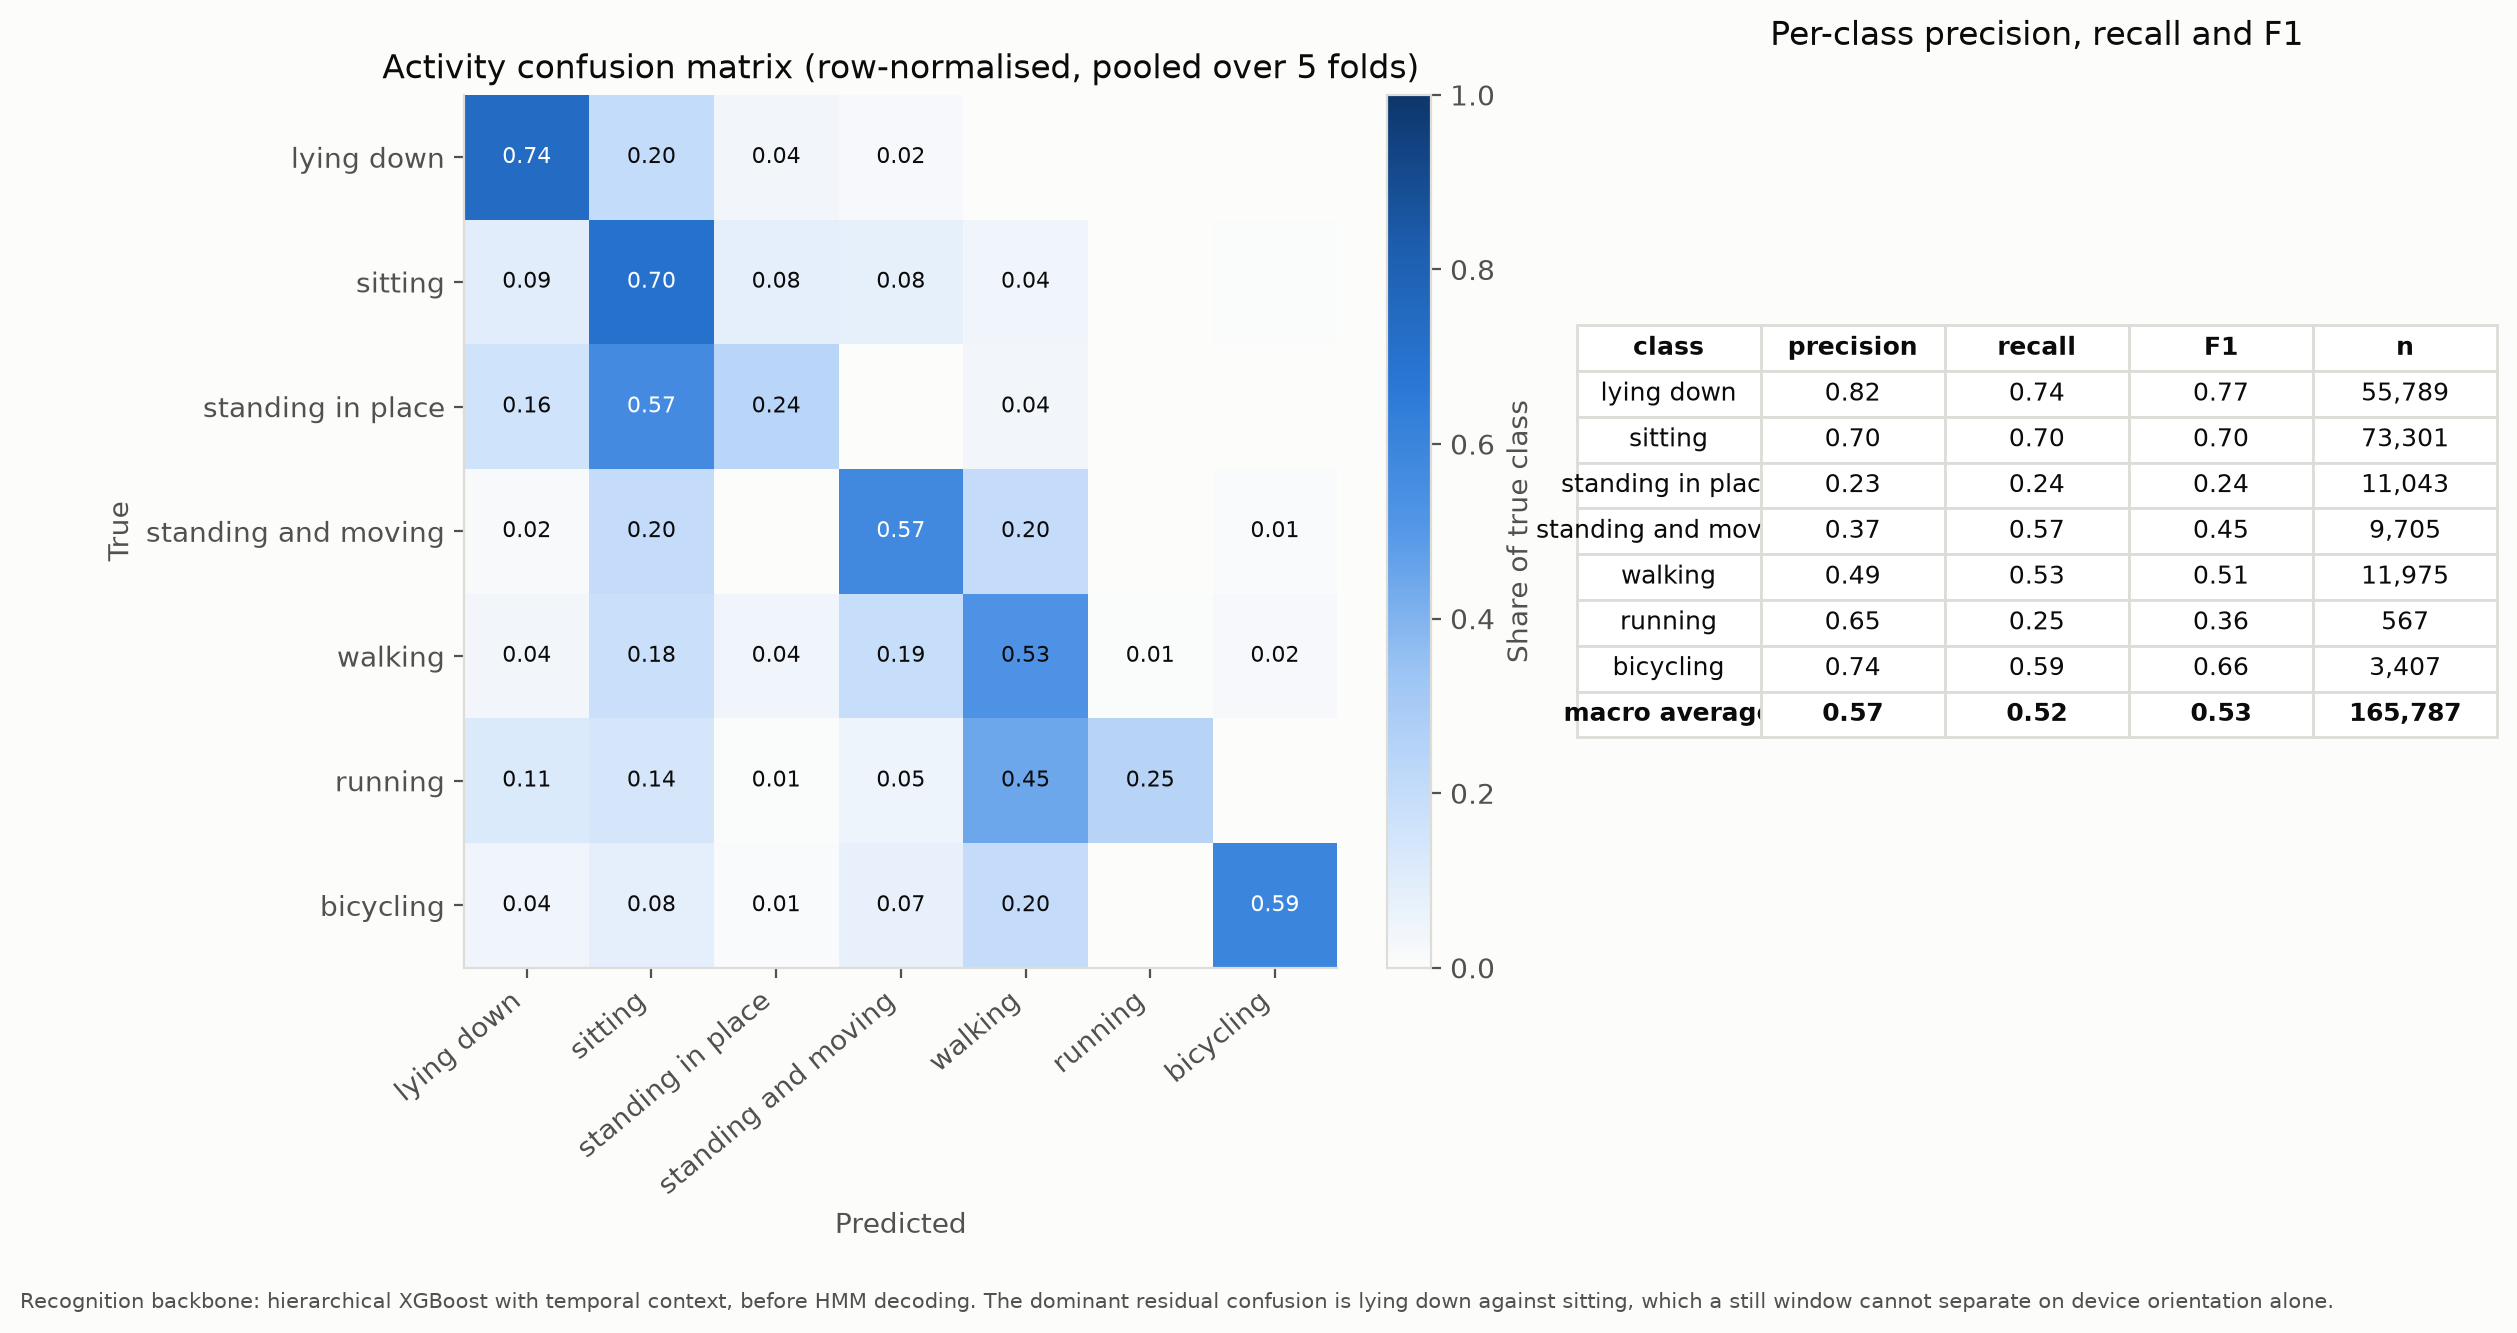
\includegraphics[width=0.62\textwidth]{figures/fig2_confusion_matrix.png}
\caption{Confusion matrix after HMM decoding. The dominant residual error is
\code{lying\_down}\,$\leftrightarrow$\,\code{sitting}: when the phone is off-body and
still, the two are not separable from accelerometer geometry alone. Temporal context
substantially mitigates this but does not remove it.}
\end{figure}

\subsection{Question answering across Tasks 1--4}

1{,}159 generated cases over the five CV folds, each scored under the rule its answer
type deserves: categorical answers by exact match; durations and onsets within
$\max(30\,\text{s},\,10\%)$; counts within $\pm 1$. \emph{Grounded} accuracy
additionally requires the cited interval to reach $\mathrm{IoU} \ge 0.5$ and the modality
and channels to match.

\begin{center}
\small
\begin{tabular}{@{}llrccc@{}}
\toprule
Task & Question type & $n$ & Answer acc. & Grounded acc. & Mean evidence IoU \\
\midrule
1 & verification    & 245 & \textbf{0.902} & 0.445 & 0.459 \\
1 & identification  & 228 & 0.474 & 0.360 & 0.466 \\
2 & comparison      &  34 & 0.882 & 0.500 & 0.534 \\
2 & duration        & 194 & 0.253 & 0.144 & 0.353 \\
2 & count           & 194 & 0.144 & 0.072 & 0.353 \\
3 & grounding       & 194 & 0.330 & 0.227 & 0.243 \\
4 & open-world      &  70 & \textbf{0.986} & \textbf{0.686} & 0.635 \\
\midrule
\multicolumn{2}{@{}l}{\textbf{overall} (macro across types)} & \textbf{1159} & \textbf{0.567} & \textbf{0.348} & --- \\
\multicolumn{2}{@{}l}{overall (micro across cases)}          & 1159 & 0.491 & --- & --- \\
\bottomrule
\end{tabular}
\end{center}

\noindent Per-fold macro answer accuracy: $0.488$, $0.595$, $0.543$, $0.621$, $0.571$.

\begin{figure}[t]
\centering

\includegraphics[width=0.49\textwidth]{figures/fig1_accuracy_by_question_type.png}
\hfill

\includegraphics[width=0.49\textwidth]{figures/fig3_accuracy_vs_strictness.png}
\caption{\textbf{Left:} answer vs.\ grounded accuracy by question type. The gap between
the two bars is the cost of having to point at the right signal, not merely to be right.
\textbf{Right:} accuracy as the grounding criterion tightens. The curve, not the single
number, is the honest summary of a grounded system.}
\end{figure}

\paragraph{Reading these numbers.} The shape is consistent and explicable.
\emph{Verification} and \emph{open-world} questions score highest because they need only
the \emph{presence} of an activity somewhere in a long recording --- robust to exactly
the boundary errors that hurt elsewhere. \emph{Duration} and \emph{count} score lowest
because both are functions of \emph{bout boundaries}: one fragmented walk becomes three
walks, which destroys a count and degrades a duration, even though every window in it was
classified correctly. This is a segmentation problem, not a classification problem, and
it is the most promising place for further work (the 180\,s merge gap is a single
constant that the reported counts depend on). \emph{Identification} at $0.474$ tracks
per-window accuracy, as it should --- it is essentially the recogniser asked one window
at a time.

\paragraph{Task 4 specifically.} The $0.986$ answer accuracy here is not evidence that
the small language model is a strong reasoner; it is evidence that the \emph{routing} is
right. Behaviour phrases that map onto the seven classes (``resting'', ``strenuous'',
``wheeled'', ``sedentary'') resolve deterministically in \code{GROUP\_PHRASES} and are
then answered by the same timeline arithmetic as Task~2, so they inherit Task~2's
reliability on presence questions. The model is invoked only for wording the rules cannot
place, and even then only as a parser.

\begin{figure}[t]
\centering

\includegraphics[width=0.7\textwidth]{figures/fig5_robustness.png}
\caption{Degradation under additive sensor noise, sample dropout, and reduced sampling
rate (fold~3, 4{,}477 windows). Accuracy falls from $0.778$ clean to $0.625$ at 1\%
additive noise and $0.520$ at 10\%, but is \emph{largely insensitive to dropout}
($0.775$ at 10\%, $0.780$ at 20\%, $0.737$ at 50\%) --- which follows directly from
clock-true resampling, since dropout is exactly what that design absorbs. Halving the
sampling rate to 12.5\,Hz costs about 13 points, most of it incurred in the first step
below 25\,Hz.}
\end{figure}

\section{Accuracy versus overhead (extra credit)}

Measured on an arm64 laptop CPU, single process, no GPU, fold~3, 36{,}087 test windows.
Feature extraction adds $0.333$\,ms per window on top of the figures below; process
peak RSS is 855\,MB.

\begin{center}
\small
\begin{tabular}{@{}lccrrrr@{}}
\toprule
Configuration & Accuracy & Macro-F1 & Features & Tree nodes & Size & Median latency \\
\midrule
full (deployed)   & 0.690 & 0.622 & 103 & 214{,}421 & 9.10\,MB & 0.366\,ms \\
pruned (62 feat.) & 0.689 & 0.589 &  62 & 191{,}702 & 8.05\,MB & 0.481\,ms \\
\textbf{shallow (edge)} & 0.547 & 0.552 & 103 & \textbf{11{,}322} & \textbf{0.95\,MB} & 0.362\,ms \\
context-free      & 0.442 & 0.412 &  40 & 110{,}998 & 4.69\,MB & 0.315\,ms \\
\bottomrule
\end{tabular}
\end{center}

\begin{figure}[t]
\centering
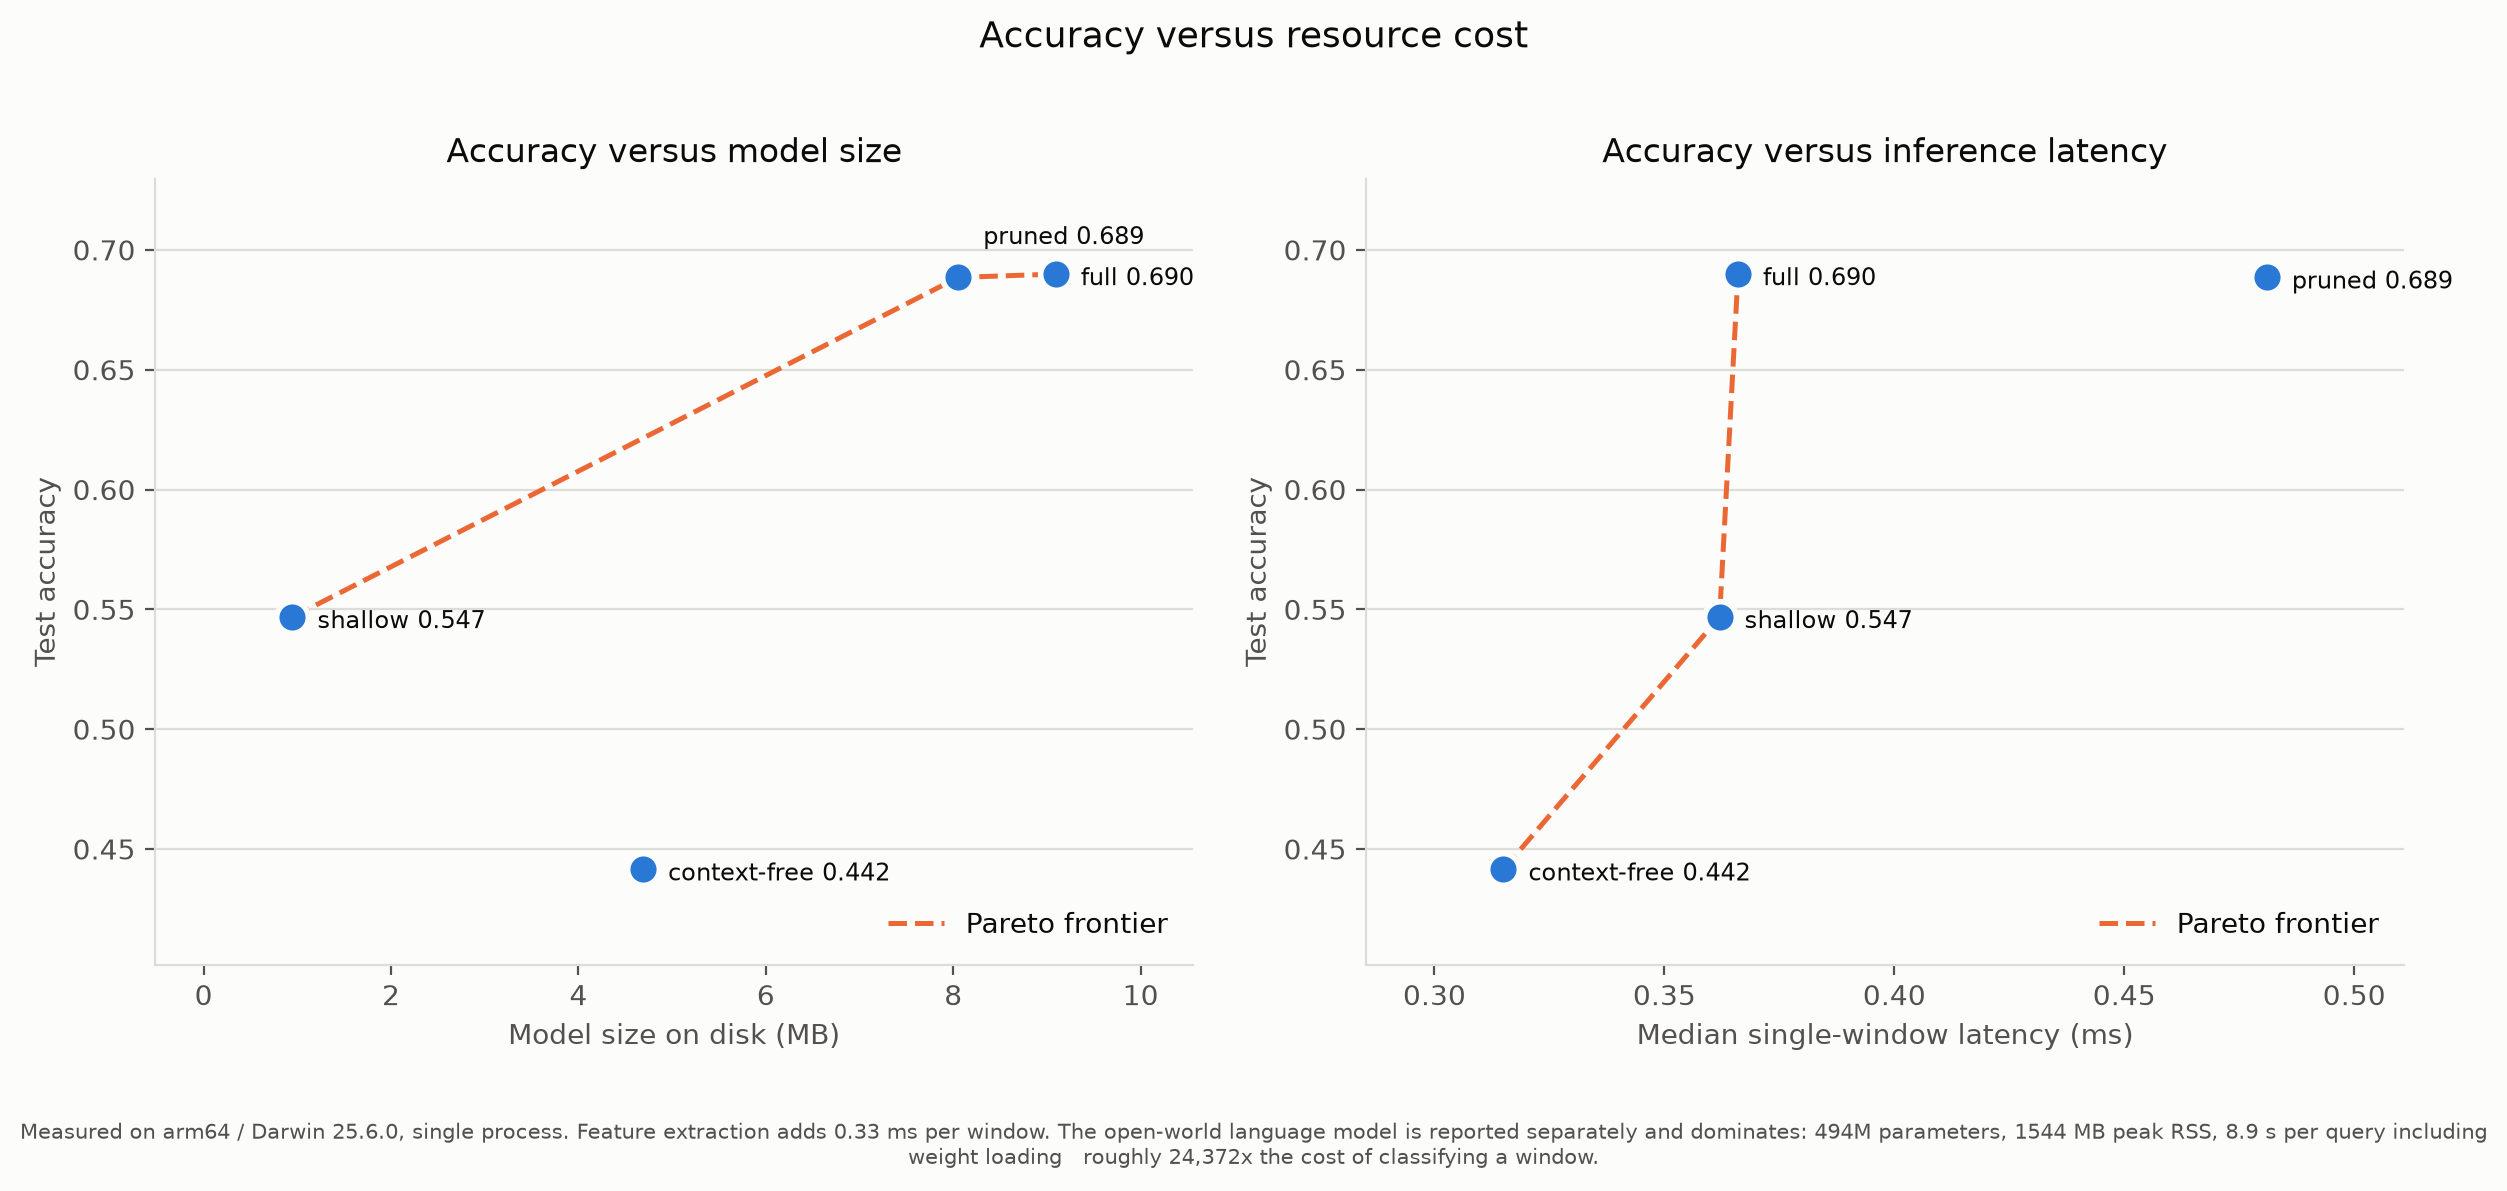
\includegraphics[width=0.68\textwidth]{figures/fig4_accuracy_vs_overhead.png}
\caption{Accuracy against model size. The useful frontier is \emph{full} and
\emph{shallow}; \emph{pruned} and \emph{context-free} are both dominated.}
\end{figure}

Three findings, each with a consequence.

\paragraph{1.\ Latency is not the binding constraint; size is.} Every configuration
classifies a window in $0.3$--$0.5$\,ms, against a 15\,s window --- a duty cycle of
roughly $3 \times 10^{-5}$. Inference time is irrelevant for any plausible wearable
deployment. What differs by an order of magnitude is the model on disk, so
\textbf{size is the axis worth trading accuracy against}, and speed is not.

\paragraph{2.\ \code{shallow} is the edge operating point.} Depth 3, 100 trees: a
$9.6\times$ reduction in size (9.10\,MB $\rightarrow$ 0.95\,MB) and a $19\times$
reduction in tree nodes, for 14 accuracy points. Note that its \emph{macro}-F1 falls only
from $0.622$ to $0.552$ --- it loses frequent-class precision faster than rare-class
recall, which makes it a better trade than the accuracy column alone suggests. It fits
comfortably in microcontroller-class flash.

\paragraph{3.\ Pruning and context removal are both bad trades.} Dropping 41 of 103
features saves $1.05$\,MB, costs nothing in accuracy --- and makes inference
\emph{slower} ($0.366 \rightarrow 0.481$\,ms median), because the pruned ensemble
compensates with deeper trees. Removing temporal context saves $4.41$\,MB and costs
$24.8$ accuracy points: the worst trade available. Context is cheap and decisive; keep it
even on constrained hardware, and cut tree depth instead.

\paragraph{The language model dominates everything, which is why it is gated.} Reported
separately because it is not comparable: 494M parameters, 1{,}544\,MB peak RSS and
$8.9$\,s per query for the 0.5B variant including weight loading (10.0\,GB and $22.6$\,s
for the 3B model we ship). That is roughly $\mathbf{24{,}000\times}$ the cost of
classifying a window. The three-stage design in \S2.7 is not an elegance argument but a
cost argument: the great majority of questions are answered by $\sim$0.16\,ms of keyword
matching plus timeline arithmetic, and never load a model at all. Latency includes cold
start, which dominates a single query; a served deployment would amortise it.

\section{Challenges faced, and how we approached them}

\paragraph{The sampling rate in the file is not the sampling rate of the data.} Our first
pipeline windowed by sample index and read cadences $15\%$ high, which made walking and
running nearly inseparable. Diagnosing this meant distrusting the data format itself and
measuring the actual inter-sample intervals --- $0.024$ to $0.077$\,s. The fix was
clock-true resampling (\S2.1); the guard against regression is
\code{tests/test\_preprocess.py}, which fails if a known 2.000\,Hz signal is read as
2.300\,Hz. This was the single highest-value bug we found, and it was invisible in
accuracy terms until we looked for it.

\paragraph{A 15-second window is sometimes information-theoretically insufficient.} Early
per-window accuracy plateaued near $0.46$ and no feature we added moved it, because
lying-still and sitting-still \emph{are the same signal}. The resolution was to stop
treating windows as independent (\S2.2, $+0.20$) --- but that created a second problem:
naive rolling statistics silently averaged across multi-hour recording gaps, inventing
continuity. Hence the 40-minute context bound and per-recording isolation, both
regression-tested.

\paragraph{The corpus does not contain the label taxonomy the brief asks for.} One
\code{OR\_standing} annotation versus two required standing classes. We chose to derive
the split explicitly from measured energy with a training-only threshold, and to
\emph{mark the provenance} of every such row, rather than quietly merge the classes or
quietly invent labels. The cost is visible and honest: \code{standing\_in\_place} is our
weakest class at $0.227$ F1, and we report it as derived wherever it appears.

\paragraph{Some labels contradict the signal.} One user's 68 running-labelled windows
have the same body-acceleration energy as lying down ($0.003$\,g) while their walking
reads $0.333$\,g --- the phone was demonstrably not on them. Combined with running being
$0.34\%$ of labelled windows, this puts a ceiling on running F1 that no model change
reaches. We chose to quantify and report this rather than filter the offending windows,
since filtering on signal-label disagreement would flatter the model with the very
examples it finds hard.

\paragraph{A small language model that produces valid output but wrong answers.} Detailed
in \S2.7. The sequence --- generate (invalid words) $\rightarrow$ constrain decoding
(valid, still wrong) $\rightarrow$ measure a larger model (9/10) --- cost a day and
produced the design's central guardrail: narrow the model's job to \emph{parsing}, keep
judgement in rules, and never let a generated token become a cited measurement.

\paragraph{PyTorch and XGBoost segfault in one interpreter.} Exit 139 on both MPS and
CPU, not fixable by \code{KMP\_DUPLICATE\_LIB\_OK}. We stopped trying to reconcile the
two runtimes and separated them by process boundary (\S3), which turned a platform
defect into the measurement apparatus the overhead analysis needed.

\paragraph{Grounded evaluation had to be built before it could be trusted.} Answer
accuracy is easy to compute and easy to be fooled by. Building a scorer with a per-type
tolerance policy and an IoU-based grounding criterion (\code{asqa/evaluate.py}) is why we
can state that our real number is $0.348$, not $0.567$ --- and why we know that counts
and durations fail through \emph{segmentation}, which is actionable, rather than through
classification, which would not have been.

\section{Known limitations}

Stated plainly, because several are properties of the data rather than of the system.

\begin{itemize}
\item \code{standing\_in\_place} is weak ($0.227$ F1) and is a derived class, not an
annotated one.
\item \textbf{Counts and durations are the weakest operations} ($0.144$ / $0.253$), and
the reported count depends on the 180\,s bout-merge constant.
\item \textbf{Running is hard} ($0.398$ F1, high variance): $0.34\%$ of windows, and some
running-labelled windows contain no motion at all.
\item \code{lying\_down}\,$\leftrightarrow$\,\code{sitting} is the dominant residual
confusion and is not fully separable from accelerometer geometry.
\item \textbf{The language-model stage is best-effort}, 9/10 on obscure wording; its
failures are visible in the explanation rather than silent.
\item \textbf{10\,GB peak RSS} when the 3B model loads; set
\code{ASQA\_SLM\_MODEL=Qwen/Qwen2.5-0.5B-Instruct} where memory binds, accepting the
documented accuracy drop.
\item Results are for smartphone-pocket-style placement in ExtraSensory; we have not
evaluated transfer to wrist-worn or chest-worn placement.
\end{itemize}

\section{Per-member contribution statement}

\noindent\textit{\small [Template --- replace with the team's actual division of work.
Percentages should sum to 100.]}

\vspace{0.5em}
\begin{center}
\small
\begin{tabularx}{\textwidth}{@{}l X r@{}}
\toprule
\textbf{Member} & \textbf{Contribution} & \textbf{Share} \\
\midrule
$\langle$Member 1$\rangle$ &
Signal layer: clock-true resampling and window rejection (\code{preprocess.py}),
the 40-feature extractor (\code{features.py}), temporal context (\code{context.py}),
the preprocessing regression tests, robustness sweeps.
& $\langle$xx\%$\rangle$ \\
\addlinespace
$\langle$Member 2$\rangle$ &
Recognition and decoding: the three-node hierarchy and probability calibration
(\code{recognise.py}), the derived standing split, user-disjoint fold construction
(\code{splits.py}), the time-aware HMM (\code{decode.py}), the accuracy-versus-overhead
benchmark.
& $\langle$xx\%$\rangle$ \\
\addlinespace
$\langle$Member 3$\rangle$ &
Evidence and interface: the timeline/evidence store (\code{timeline.py}), intent parsing
and the six answer handlers (\code{intent.py}, \code{answer.py}), the gated language-model
stage and its process isolation (\code{slm.py}, \code{slm\_worker.py}), the grounded
QA evaluator, the dashboard, this report.
& $\langle$xx\%$\rangle$ \\
\midrule
\multicolumn{2}{@{}l}{\textit{Joint}} & \\
\multicolumn{3}{@{}p{0.95\textwidth}}{\small The four-layer architecture and the
evidence-flows-up invariant were agreed jointly before implementation. All members
participated in the small-language-model parsing study, the design review of the
grounded-accuracy criterion, and final integration testing.} \\
\bottomrule
\end{tabularx}
\end{center}

\section{Mandatory AI-use disclosure}

\noindent\textit{\small [Template --- replace every bracketed field with what the team
actually did. Be specific; a vague disclosure is worse than a detailed one.]}

\vspace{0.5em}
\noindent\textbf{Tools used.} $\langle$Tool name and version, e.g.\ ``Claude Code
(Opus), ChatGPT (GPT-x), GitHub Copilot''$\rangle$.

\vspace{0.4em}
\noindent\textbf{What they were used for.}
\begin{itemize}
\item \emph{Code:} $\langle$e.g.\ scaffolding of module boilerplate and CLI argument
parsing; drafting \code{<names of files or functions>}; refactoring for readability;
writing regression tests from specifications we wrote$\rangle$.
\item \emph{Debugging:} $\langle$e.g.\ diagnosing the XGBoost/PyTorch segfault; tracing
the index-vs-timestamp resampling error$\rangle$.
\item \emph{Analysis and writing:} $\langle$e.g.\ drafting and copy-editing this report
from numbers and notes we produced; formatting LaTeX tables$\rangle$.
\item \emph{Not used for:} $\langle$e.g.\ choosing the architecture; selecting features;
producing or adjusting any reported number$\rangle$.
\end{itemize}

\vspace{0.4em}
\noindent\textbf{Verification.} $\langle$State how AI-assisted output was checked: e.g.\
every AI-written function was read line by line by a named member; all reported metrics
were regenerated from committed code by running the documented pipeline; the regression
tests in \code{tests/} were written to pin behaviour we had verified by hand.$\rangle$

\vspace{0.4em}
\noindent\textbf{Responsibility.} All team members have read and understood every line of
the submitted code and take full responsibility for its correctness. No result in this
report was produced, estimated, or edited by a language model; every number is emitted by
committed code and stored in \code{outputs/evaluation/}.

\begin{thebibliography}{9}
\small
\bibitem{vaizman2017}
Y.~Vaizman, K.~Ellis, and G.~Lanckriet.
``Recognizing Detailed Human Context In-the-Wild from Smartphones and Smartwatches.''
\emph{IEEE Pervasive Computing}, 16(4):62--74, 2017.
\url{http://extrasensory.ucsd.edu/}

\bibitem{qwen}
Qwen Team, Alibaba Cloud. \emph{Qwen2.5-Instruct} (Apache~2.0). Used for Task~4
open-world question parsing.

\bibitem{xgboost}
T.~Chen and C.~Guestrin. ``XGBoost: A Scalable Tree Boosting System.''
\emph{KDD}, 2016.

\bibitem{libs}
NumPy, SciPy, scikit-learn, PyTorch, Hugging Face Transformers, Matplotlib.
\end{thebibliography}

\appendix
\section{Reproducing every number in this report}

\begin{quote}\small
\begin{verbatim}
python -m asqa.preprocess              # raw .dat -> 25 Hz windows, cached per user
python -m asqa.splits                  # rare-class-aware, user-disjoint folds
python -m asqa.recognise --build-features
python -m asqa.recognise --cv          # context-free + context-aware, per fold
python -m asqa.decode --cv             # HMM decoding, both variants, both methods
python -m asqa.evaluate --cv           # QA scoring by question type
python -m asqa.benchmark --fold 3      # size, latency, memory, operating points
python -m asqa.robustness --fold 3     # noise / dropout / sampling-rate sweeps
python -m asqa.figures                 # the five figures in this report
\end{verbatim}
\end{quote}

\noindent The JSON behind every table is committed under \code{outputs/evaluation/}:
\code{recognition\_cv.json} (\S4.1), \code{decode\_cv.json} (\S4.1),
\code{qa\_cv.json} (\S4.2), \code{benchmark.json} (\S5), \code{robustness.json}
(Fig.~4). The fold assignment is committed as \code{outputs/folds\_w15.json}, so the
split behind the reported numbers is exactly reproducible.

\section{Example answer}

\begin{quote}\small
\begin{verbatim}
Query: "How long was the user walking?"

Answer:             11559 seconds
Activity/Event:     walking
Evidence:
    Timestamp(s):      25485 to 26160, 28545 to 30300, 163563 to 165558,
                       183483 to 184278, 202223 to 202958, 255083 to 256247
                       (+11 shorter intervals totalling 4440 s)
                       (seconds from start)
    Sensor Modality:   Accelerometer, Gyroscope
    Sensor Channel(s): All
Explanation:        Walking was detected in 17 intervals spanning 11559 s in
                    total (193 min). The recording samples about 23% of
                    wall-clock time, so this span rests on 3075 s of directly
                    observed sensor data.
\end{verbatim}
\end{quote}

\end{document}
